\documentclass[10pt]{beamer}

\usetheme[progressbar=frametitle]{metropolis}
\usepackage{appendixnumberbeamer}

\usepackage{booktabs}
\usepackage[scale=2]{ccicons}
\usepackage{xeCJK}
\usepackage{amsmath}

\usepackage{pgfplots}
\usepgfplotslibrary{dateplot}

\usepackage{xspace}
\newcommand{\themename}{\textbf{\textsc{metropolis}}\xspace}
\setbeamercolor{background canvas}{bg=white}
\title{Yelp Data Prediction}
\subtitle{Preliminary Analysis}
% \date{\today}
\date{}
\author{Yifan Li, Chenlai Shi, Jianmin Chen}
\institute{Monday Group 1}
% \titlegraphic{\hfill\includegraphics[height=1.5cm]{logo.pdf}}

\begin{document}

\maketitle

\begin{frame}{Data Overview}
\textbf{Yelp training data} 

Over 1,500,000 rows with no missing values

\textbf{Variables to be excluded}
\begin{itemize}
    \item[-] Name, City, Latitude, Longitude
    
    Too many different levels.
    
    City: over 600 levels
    
    Name: over 30,000 levels
\end{itemize}

\textbf{Variables to be used}

Text, Category, Stars, Date
\end{frame}

\begin{frame}{Date: Date Description}
\textbf{Date}
\begin{figure}
    \centering
    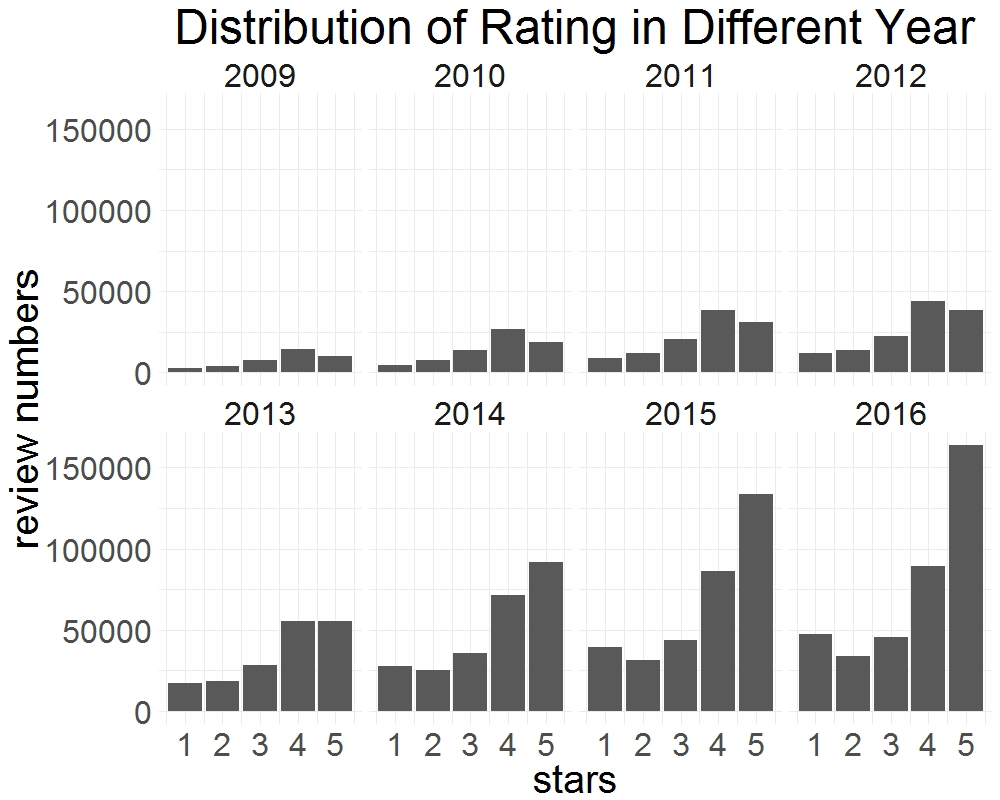
\includegraphics[scale=0.3]{date.jpeg}
\end{figure}    
    
\end{frame}

%2---------------------------------------------------------------------------------------

\begin{frame}{Data Cleaning}


\begin{itemize}

	\item[1] Abbreviation and Special Symbol

	\item[2] Non-English

	\item[3] Negative Sentences
	
	\item[4] Punctuation

\end{itemize}

\end{frame}

%----------------------------------------------------------------------------------------

%2.1----------------------------------------------------------------------------------------

\begin{frame}{Text: Abbreviation and Special Symbol}

\begin{table}[ht]

\centering % used for centering table
\begin{tabular}{c c} % centered columns (4 columns)
\hline %inserts double horizontal lines
Origin & Now \\ [0.5ex] % inserts table
%heading
\hline % inserts single horizontal line
n't &   not\\  
's &   is\\  
've &   have\\  
'd &   would\\  
'm &   am\\  
Ive &  I have\\  
cannot &  can not\\
$\backslash$n & Space \\
\hline %inserts single line
\end{tabular}
\label{table:nonlin} % is used to refer this table in the text
\end{table}
\end{frame}

%2.1---------------------------------------------------------------------------------------

\begin{frame}{Text: Abbreviation and Special Symbol}


\begin{table}[ht]
\caption{Example} % title of Table
\centering % used for centering table
\begin{tabular}{c c c} % centered columns (4 columns)
\hline %inserts double horizontal lines
Line & Origin & Now \\ [0.5ex] % inserts table
%heading
\hline % inserts single horizontal line
3 & Long story short.$\backslash$n$\backslash$nBunch ... & Long story short.  Bunch \\
6 & ... We didn't catch her ... & ... We did not catch her ...  \\  
8 & ... It's super clean ... & ... It is super clean...  \\  
\hline %inserts single line
\end{tabular}
\label{table:nonlin} % is used to refer this table in the text
\end{table}
\end{frame}

%----------------------------------------------------------------------------------------

%2.2---------------------------------------------------------------------------------------

\begin{frame}{Text: Non-English}

\begin{table}[ht]
\caption{Example} % title of Table
\centering % used for centering table
\begin{tabular}{c c} % centered columns (4 columns)
\hline %inserts double horizontal lines
Line & Review \\ [0.5ex] % inserts table

\hline % inserts single horizontal line
24 & 2ème arrêt au Barbù et nous avons vécu une  ... \\  
1167 & Corriente, sucio, y mal servicio. El cocinero  ... \\  
2580 & アリゾナ 最後に 良い旅の想い出の締めくくり  ... \\  
3750 & 家から最寄りで食べに行けるベトナム料理 ...  \\  
\hline %inserts single line
\end{tabular}
\label{table:nonlin} % is used to refer this table in the text
\end{table}
\end{frame}

%----------------------------------------------------------------------------------------

%2.2---------------------------------------------------------------------------------------

\begin{frame}{Text: Negative Sentences}

\textbf{Inverter: } not, never, lack, no
\newline
\newline
\textbf{Before:}\\
Seriously can not stand this McDonald is. They NEVER get my order right.
\newline
\newline
\textbf{After:}\\
seriously can not notstand notthis notmcdonald notis. they never notget notmy notorder notright.\\

\end{frame}

%----------------------------------------------------------------------------------------
\begin{frame}{Feature Engineering}
   \begin{figure}
    \centering
    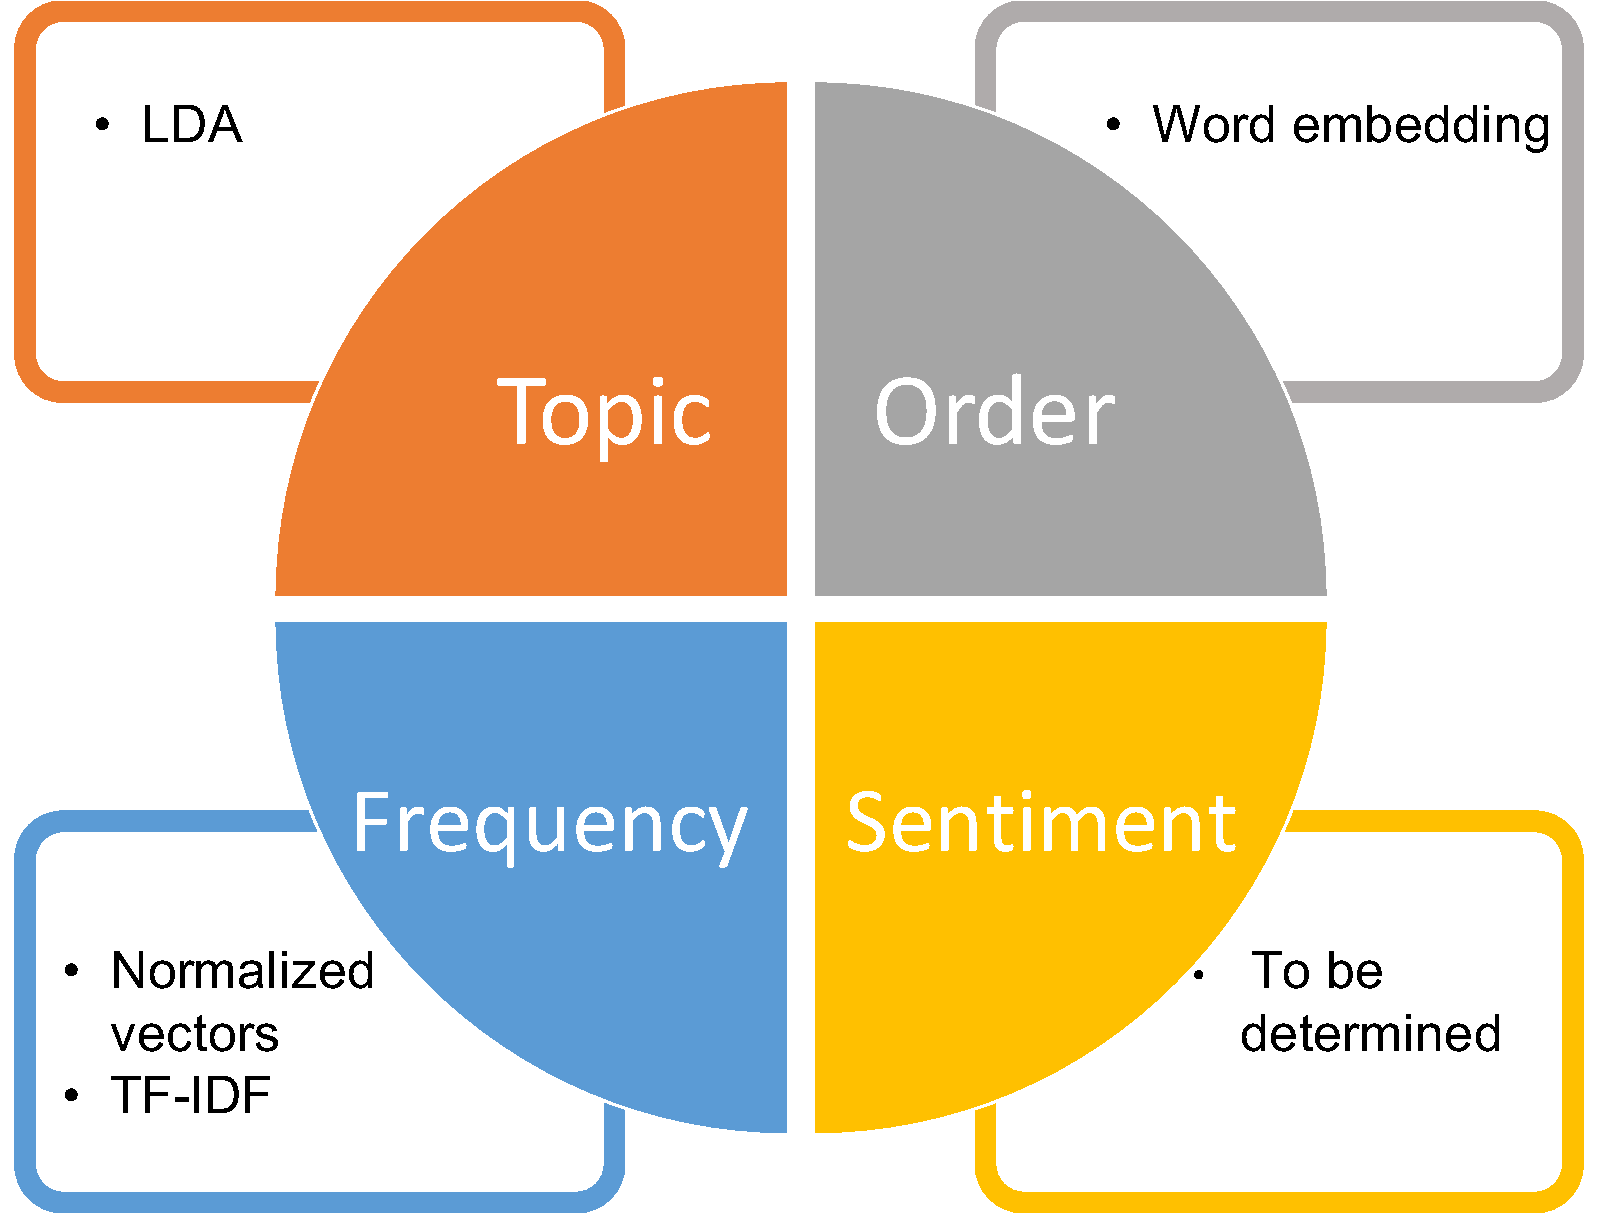
\includegraphics[scale=0.35]{feateng.pdf}
    
\end{figure}     
\end{frame}
\begin{frame}{Dimension Reduction}
\begin{itemize}
	\item Singular value decomposition
	\item Chi-square test
	\item Tree-based feature selection
	\item Removing features with low variance
\end{itemize}
\end{frame}

\begin{frame}{Dimension Reduction}
\begin{figure}[htbp]
\centering
\setlength{\belowcaptionskip}{2pt} 
\begin{minipage}[t]{0.48\textwidth}
\centering
\setlength{\belowcaptionskip}{1pt} 
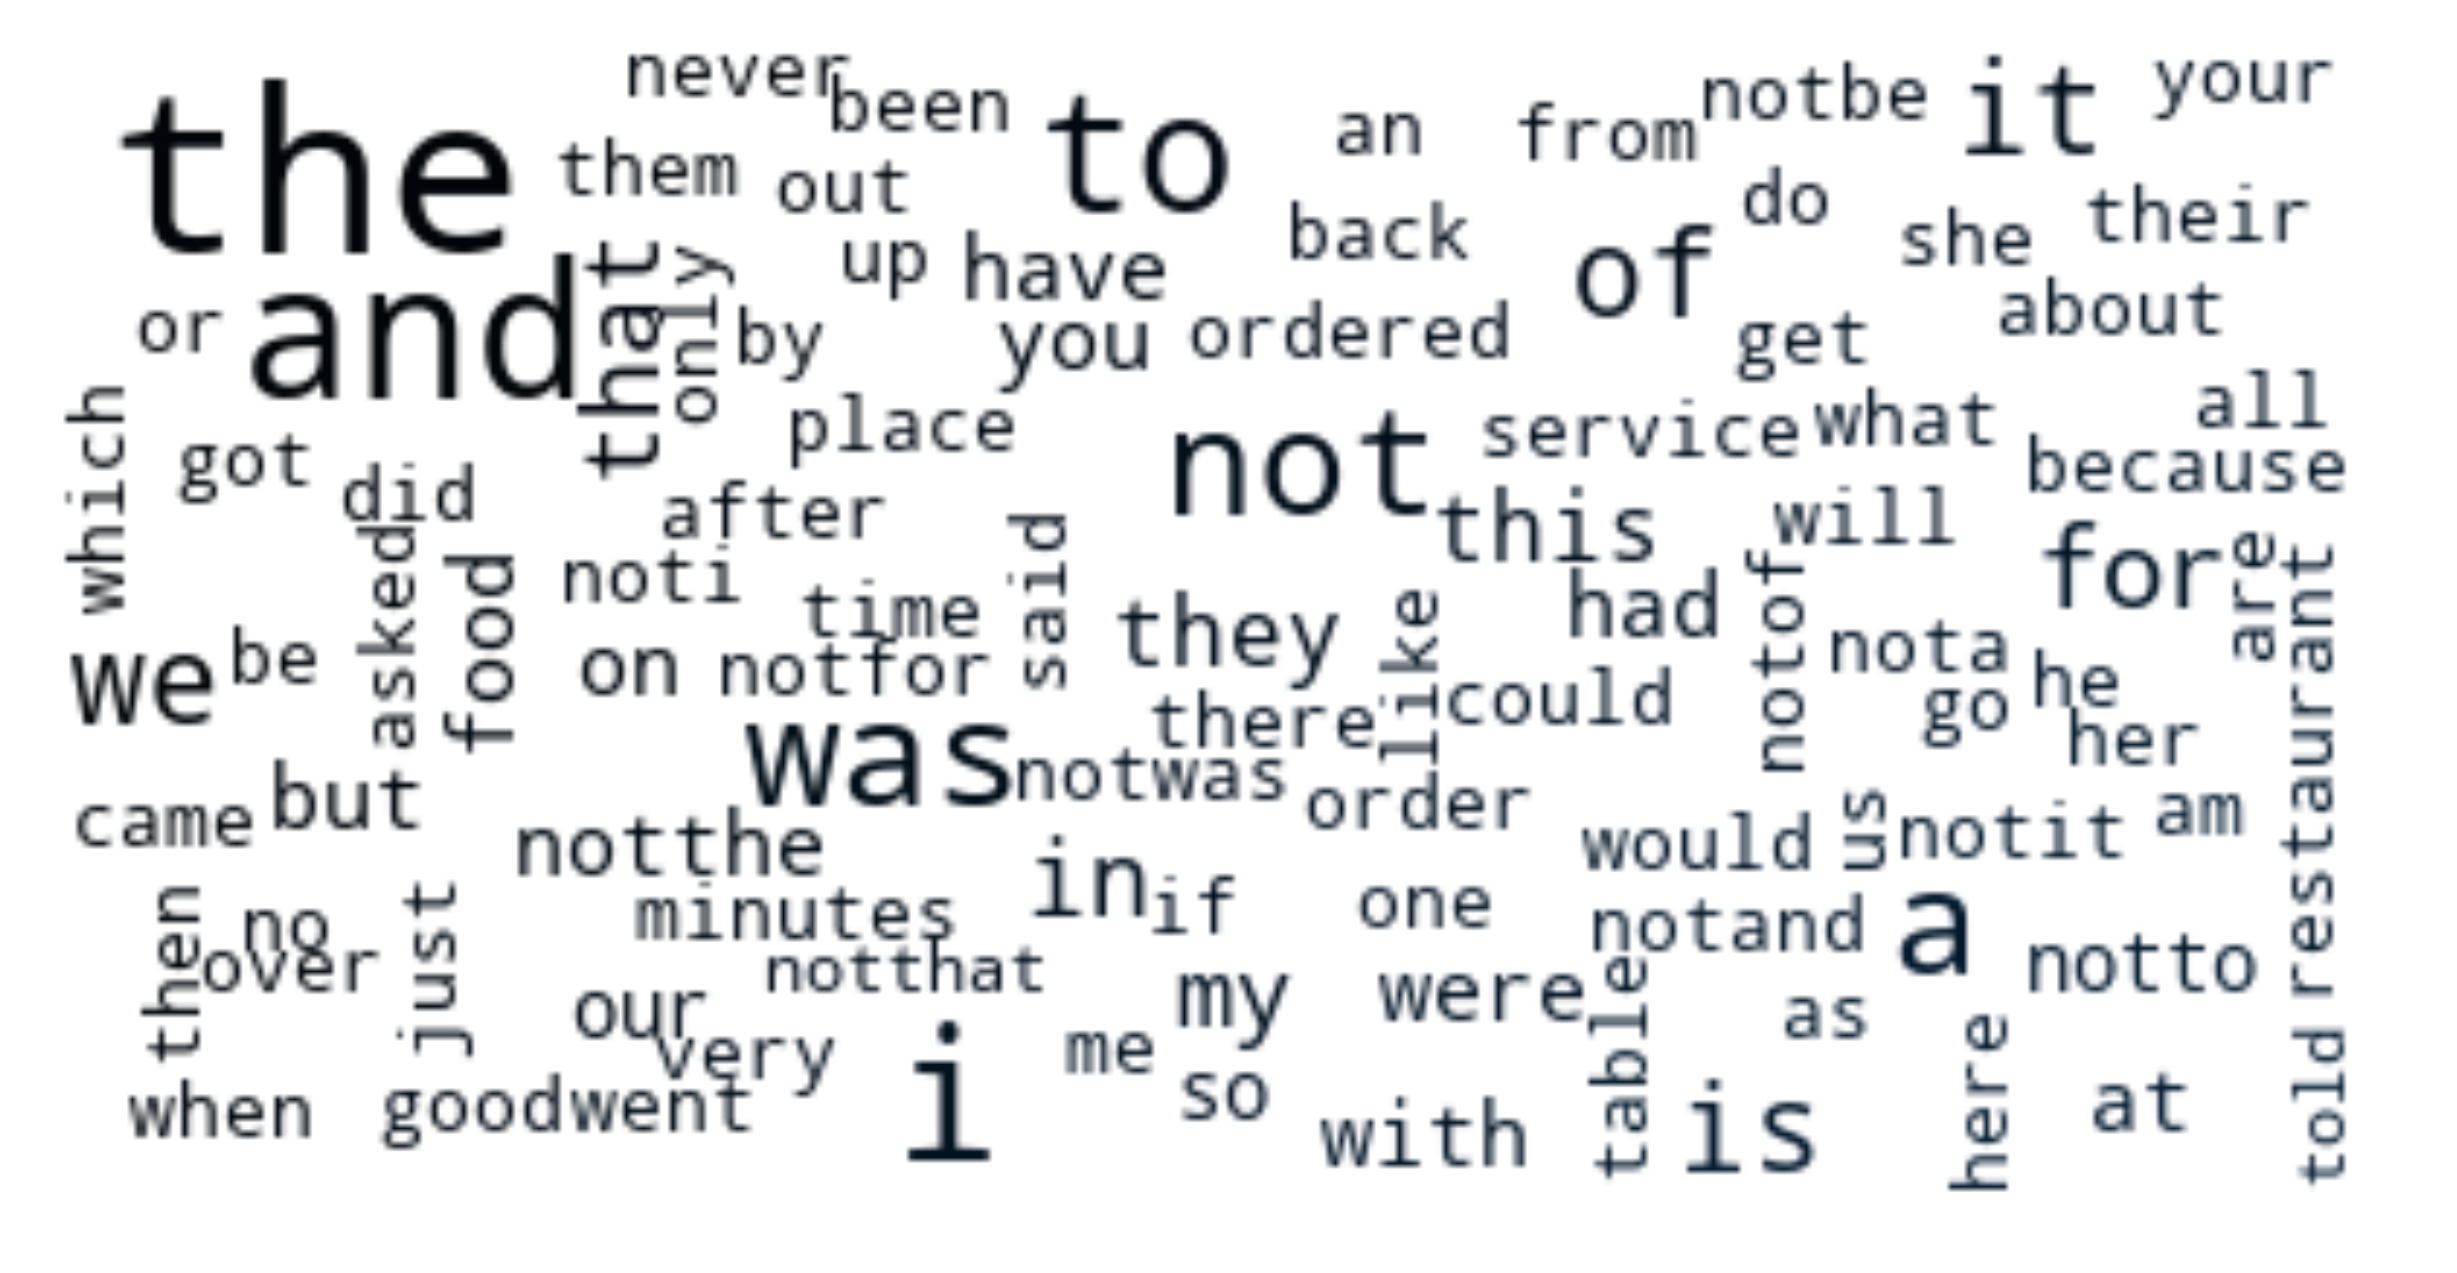
\includegraphics[width=5.1cm,height=5cm]{dist1_ori.png}
\caption{Before}
\end{minipage}
\begin{minipage}[t]{0.48\textwidth}
\centering
\setlength{\belowcaptionskip}{1pt} 
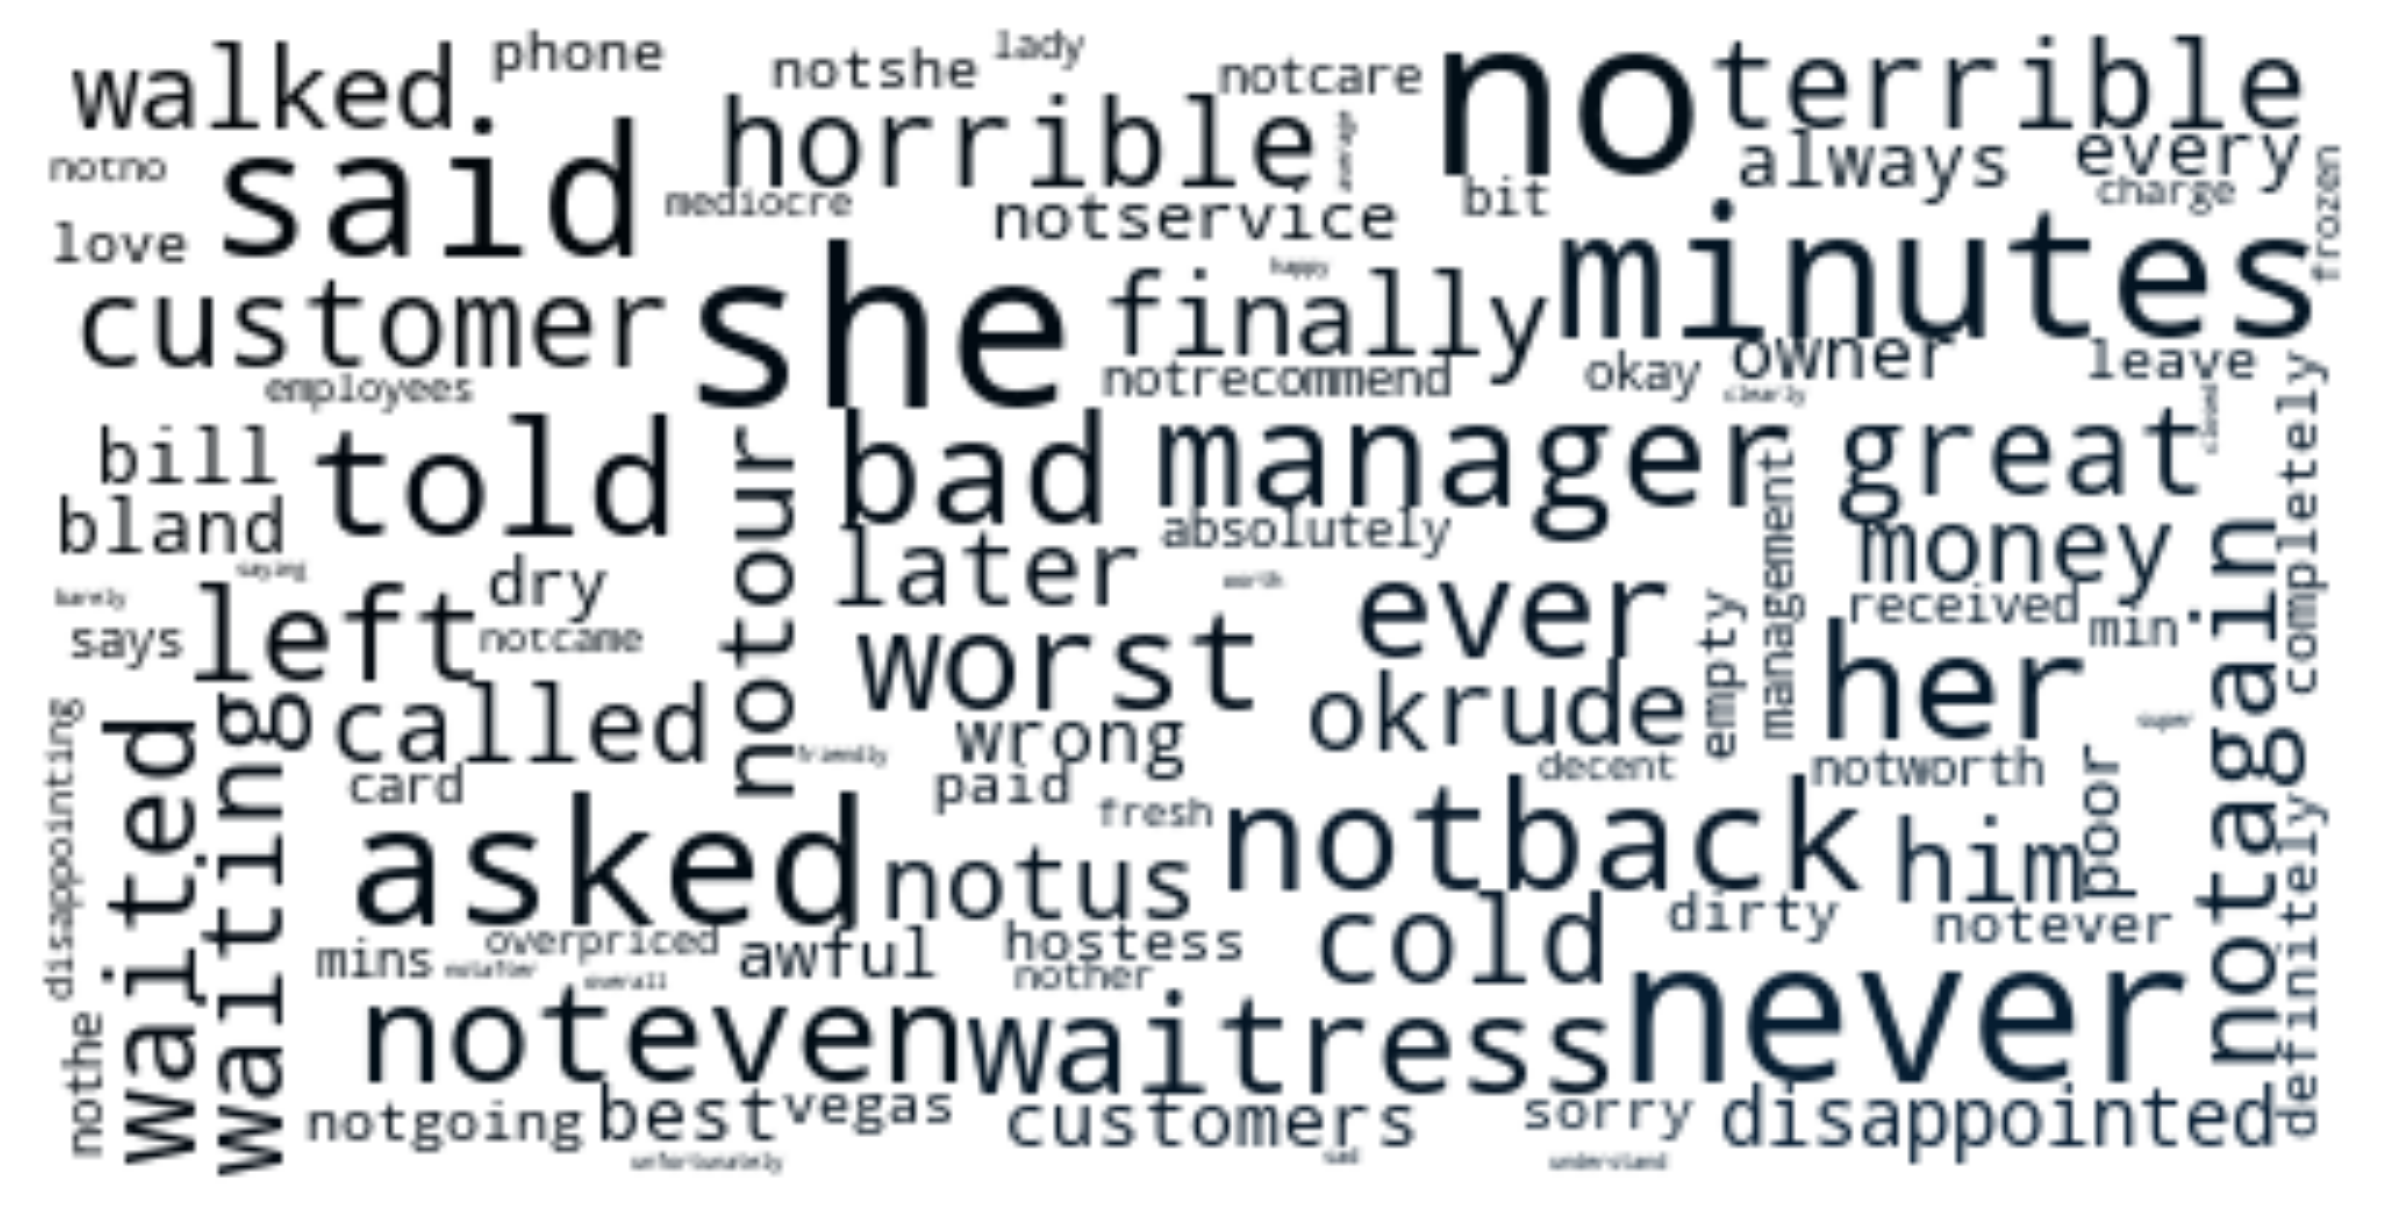
\includegraphics[width=5.1cm,height=5cm]{dist1.png}
\caption{After}
\end{minipage}
\end{figure}
$$\textbf{Word Clouds for 1-star Review}$$
\end{frame}



\begin{frame}{Dimension Reduction}
\begin{figure}[htbp]
\centering
\begin{minipage}[t]{0.48\textwidth}
\centering
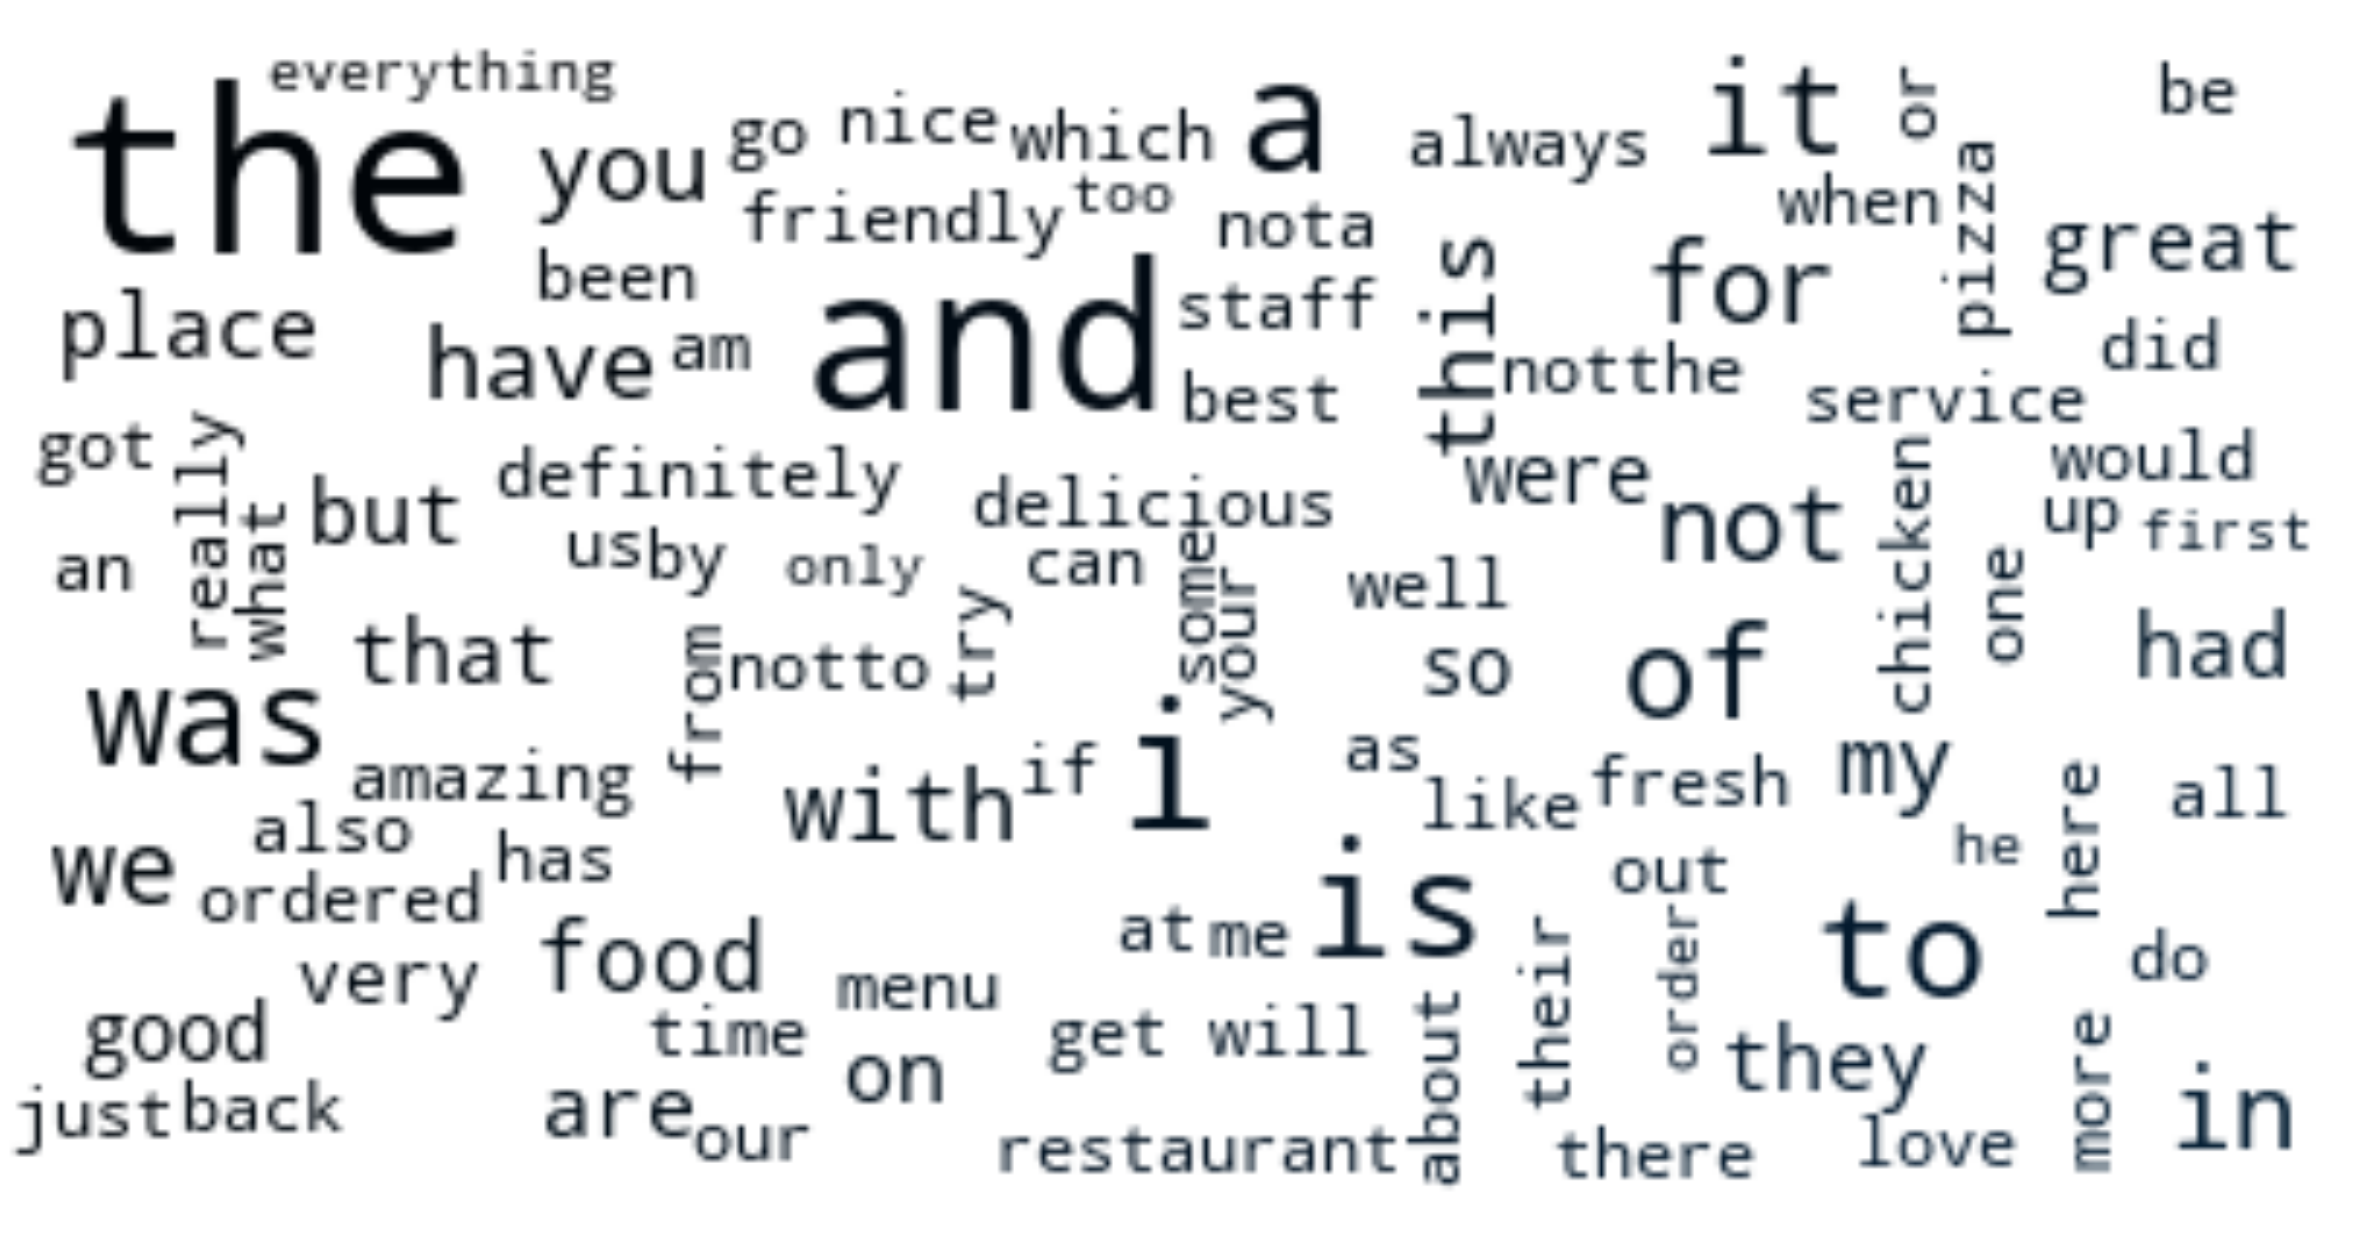
\includegraphics[width=5.1cm,height=5cm]{dist5_ori.png}
\caption{Before}
\end{minipage}
\begin{minipage}[t]{0.48\textwidth}
\centering
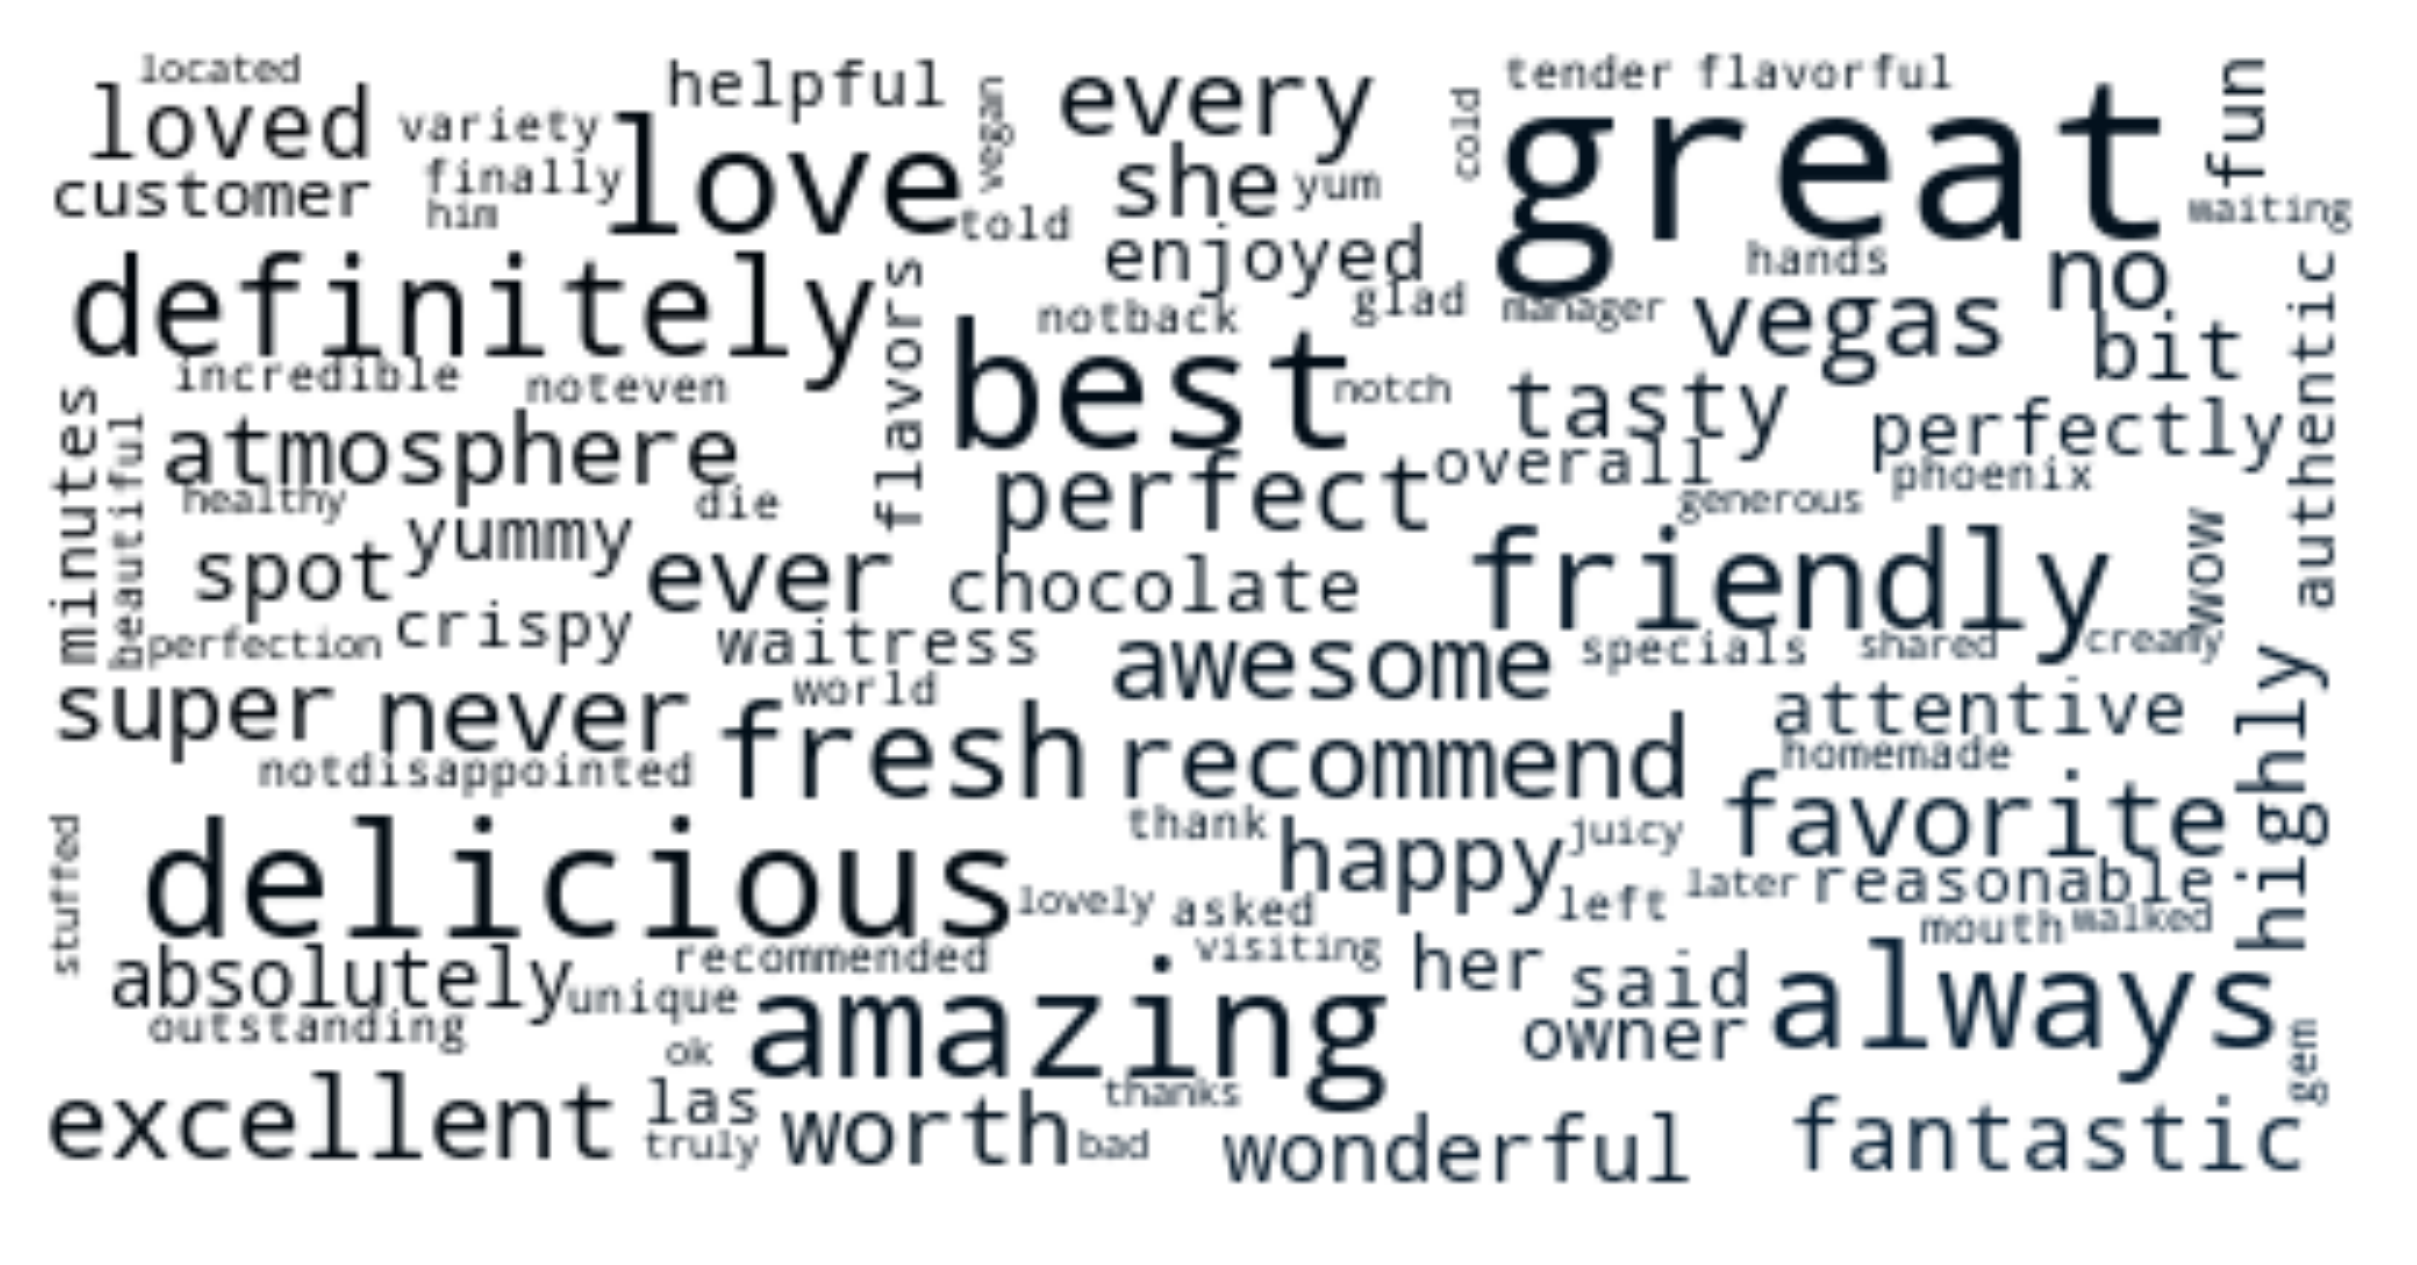
\includegraphics[width=5.1cm,height=5cm]{dist5.png}
\caption{After}
\end{minipage}
\end{figure}
$$\textbf{Word Clouds for 5-star Review}$$   
\end{frame}

\begin{frame}
\Huge{\centerline{Thank You!}}
\end{frame}
\end{document}
